\IEEEraisesectionheading{\section{Introduction}}
\IEEEPARstart{O}{n-device} training Neural Networks (NNs) has been a crucial catalyst towards privacy-preserving and personalized mobile intelligence.
There exist numerous applications: input prediction personalization ~\cite{xu2018deeptype}, sequential recommendation system ~\cite{han2021deeprec}, video analytics ~\cite{bhardwaj2022ekya}, voice assistant wake-up service ~\cite{siri}, etc.
Due to its huge resource demand, substantial prior literature~\cite{huang2023elastictrainer, xu2022mandheling, 10.1145/3295500.3356156, mercury2021sensys, 10.1145/3384419.3430716, zhu2023pockengine, tflite, tfjs, MNN} have attempted to alleviate its resource tension on mobile devices.

Recently, Parameter-Efficient Training (PET) methods such as adapter~\cite{houlsby2019parameter, rebuffi2017learning} and LoRA~\cite{hu2021lora} have been widely recognized as an effective training paradigm.
Freezing most of the pre-trained weights, PET achieves competitive accuracy by adjusting only a tiny portion (e.g., $\le$1\%) of parameters compared to fully fine-tuning the model.
%textbf{\textit{a few}} \textbf{\textit{predefined}} parameters (e.g., < 1\% trainable parameters by inserting Adapters~\cite{houlsby2019parameter, rebuffi2017learning}).
Thereby, PET can efficiently deploy a shared foundation NN~\cite{yuan2023rethinking, yang2023edgefm} to multiple downstream tasks on devices, with only a few plug-and-play parameters.
As will be shown in $\S$\ref{subsec:pre-measure}, it also reduces the training overhead including memory footprint and data labels --- two scarce resources on mobile devices.
It could even offer
enhanced data security by leveraging TEE to protect the plugged parameters~\cite{zhang2023no}.

% \begin{figure}[!t]
    
    \raggedleft
    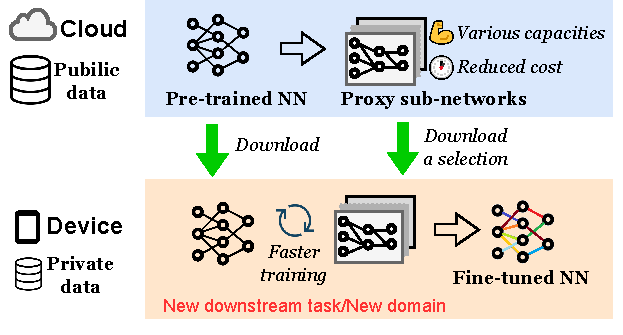
\includegraphics[width=0.98\linewidth]{figs/intro.drawio.pdf}
    
    \caption{How \sys works.}
    \label{fig:sketch map of PEFT}
    
\end{figure}


% Neural Networks (NNs) are a key enabler for mobile intelligence.
% Although NNs pre-trained on public large-scale cloud datasets have shown impressive foundational representational ability and generalization prowess, they still need on-device training to adapt to versatile and dynamic environmental domains or downstream tasks. 
% Many mobile/edge applications perform on-device fine-tuning, such as input personalization service ~\cite{xu2018deeptype}, sequential recommendation system ~\cite{han2021deeprec}, video analytics ~\cite{bhardwaj2022ekya}, voice assistant wake-up service ~\cite{siri}, etc.
% As such, on-device adaptation/personalization has recently become an eyeball-grabbing research domain ~\cite{}.

% On-device training is known to be much more resource-intensive than inference and often unaffordable on mobile devices. 
% \mwx{People might think fine-tuning is lightweight (as compared to pre-training). Show some numbers to back up?}
% For instance, using Raspberry Pi 4 to train Vision Transformer (ViT\_base) on Caltech-256 dataset can take over a month.
% Even on stronger devices with GPUs such as Nvidia Jetson TX2, the training on each image could still take over 30 seconds.
% Training ResNet-50 with one batch (batch size 32) takes 4.6 GB memory and 36.4 seconds on the smartphone MI 10. 
% The consumed energy equals to watching a 1080P-definition video for 111.2 seconds ~\cite{}.
% Fine-tuning tasks typically need thousands of iterations to converge, so the end-to-end training could take hours or days with unbearable energy consumption.
% Fortunately, recent advances in ML algorithms show that, with a large pre-trained NN, we can only update very few parameters (e.g., < 1\%) while achieve the similar accuracy, namely parameter-efficient training (PET).
% Popular PET algorithms include Linear probing ~\cite{}, Last $K$ layers ~\cite{}, Adapters ~\cite{}, LoRA ~\cite{}, and P-tuning ~\cite{}, etc. 
% PET methods are also scalable: the larger pre-trained model, the fewer parameters needing to be updated.

% According to our measurement in $\S$\ref{subsec:pre-measure}, PET indeed can effectively save storage and the need for data labels that are difficult to obtain on devices. 
% For instance, PET methods can achieve up to 17.32\% accuracy improvement with scarce data labels, and significantly reduce storage overhead by 5.6$\times$ when adapting to 6 different downstream tasks.
% Those factors take a giant step to make on-device fine-tuning practical. 

% \mwx{Highlight the issue in a separated paragraph}
However, such parameter efficiency does not translate coequal to time efficiency.
For instance, when fine-tuning ResNet50~\cite{he2015deep} on a MI 10 smartphone,
%using the Caltech-256~\cite{c256} dataset,
PET methods with less than 1\% trainable parameters still consume up to 96\% and on average 65\% of the training time compared to traditional full-model fine-tuning ($\S$\ref{subsec:pre-measure}, Figure~\ref{fig:time_measure}).
Such long training time results in more energy consumption, compromised user experience and delayed personalization service.
% \mwx{Talk about the consequences of long training time: more energy consumption, compromising user experience, delayed personalization service..}
Diving into the reason, we find out that the frozen layers dominate the training time (both forward pass and backward pass).
% \mwx{The frozen layers computing includes forward pass, but backward? Make it clear.}
For instance, when training Vision Transformer (ViT\_base)~\cite{dosovitskiy2021an} on NVIDIA Jetson TX2 with PET methods, the frozen layers account for 96.34\%–-99.59\% of the computation time (Table~\ref{table-frozenvstrainable}).
This observation provides a key opportunity that, as the compute-intensive layers are frozen during training, we can approximate them with cheaper ones (dubbed as \textit{Proxy sub-networks}, or \textit{subnets} in short).
% \mwx{Does't flow here. How about position it as one major challenge after introducing our key idea of subnet?}
% Yet, a simple, static replacement strategy could result in nontrivial degradation of convergence accuracy.
% For instance, replacing a ViT\_base with a structurally identical network that has significantly fewer FLOPs (e.g., < 50\%) for fine-tuning on the DTD dataset would result in a 29.11\% decrease in accuracy ($\S$\ref{subsec:ablation}, Figure ~\ref{fig:static}), and this number would further increase on more complex datasets.
% \mwx{say something like: while such approximation has been exploited for inference speedup, we are the first to apply it to on-device training.}
% While such approximation has been exploited for inference speedup~\cite{torchpruninggithub, krishnan2019structural}, we are the first to apply it to on-device training.

% To fully leverage this opportunity and further tap into the potential of parameter efficiency, we propose \sys, the first framework that effectively speeds up on-device PET through frozen-layer approximation.
% % \mwx{briefly describing the system model of \sys? goal is time-to-accuracy; cloud-device collboration; etc.}
% Its design goal is to achieve a better time-to-accuracy for on-device PET.
% To realize this goal, it works through cloud-device collaboration, leveraging the rich pre-training data to achieve NN approximation on cloud.

%\textbf{Challenge: static approximation significantly compromises accuracy.}
The main challenge in accelerating PET through NN approximation is that a \textit{simple, static replacement strategy} could result in nontrivial degradation of convergence accuracy.
For instance, approximating the frozen layers of a ViT\_base with a structurally identical network that has significantly fewer FLOPs (e.g., < 50\%) for fine-tuning on the DTD~\cite{dtd} dataset would result in a 29.11\% decrease in accuracy ($\S$\ref{subsec: sensitivity}, Figure ~\ref{fig:static}), and this number would further increase on more complex datasets~\cite{c256, ImageNet2012, ImageNet-21K}.
% \mwx{Provide intuitive reasons that echo to our design.}
This arises from two aspects: one is the error between the approximated network and the original network; the other is the compromised generalization ability due to the decreased model capacity.
% \mwx{last sentence needs to be polished}

In response, this work presents \sys, the first fast PET framework for mobile devices.
Instead of statically approximating the frozen layers during PET, the key idea of \sys is \textbf{data-aware dynamic approximation and routing.}
It's based on a key insight that the approximation of frozen layers must be more fine-grained, i.e., \textit{be dynamic for different training samples} during on-device training due to the high diversity of real-world data~\cite{ijcai2017p0735, he2019data, 10.1145/3495243.3517016, mercury2021sensys, canel2019scaling, 10.1145/2972413.2972423, 10.1145/3241539.3241557, pmlr-v162-mindermann22a, huang2018multiscale}.
More specifically, the training data exhibits opportunistic diversity in two unique aspects: \textit{difficulty} and \textit{importance}.
Difficulty is that some training samples are intrinsically easier to extract accurate and informative features from.
Importance is that some non-trivial training samples can facilitate faster convergence and better generalization.
We define them in our system model and show their ubiquitous presence in $\S$\ref{subsec:Opportunity: Training Data diversity}.

Realizing the above design needs to tackle two crucial challenges.
First, training-oriented subnets are hard to acquire: they must be with low approximation-induced accuracy loss, fast on-device execution speed, and a vast latency-accuracy trade-off space.
Second, as will be shown in $\S$\ref{subsec:Opportunity: Training Data diversity}, perceiving data diversity is non-trivial: data importance is stateful, and data difficulty is stateless but posterior. 
Online perceiving data diversity brute-force and forming routing strategy introduce undesirable extra time overhead.

\sys incorporates a two-stage design akin to prior literature~\cite{wen2023adaptivenet, Fang_2018, wang2022melon}:
on cloud (offline), it pre-generates the approximated subnets through public data;
on devices (online), it finetunes the models by judiciously routing the data to proper subnets.
%on cloud once and deploying these subnets along with the original NN to devices to assist on-device training. 
Specifically, the aforementioned challenges are tackled in the following two stages: the on-cloud pre-approximation and the on-device data-aware routing.

In the first stage, \sys employs a pruning-based fine-grained approximation method.
By gradually and structurally removing various components from the original NN, this method generates subnets with faster on-device execution speed.
The design differs significantly from prior inference-oriented pruning-based NN approximation~\cite{torchpruninggithub, krishnan2019structural}, since:
(1) It redesigns the pruning specification for PET, ensuring that the pruned NN structure is compatible with the parameter efficiency of the original NN.
(2) It recognizes that the requirements of NN approximation for training are more stringent (i.e., latent space alignment instead of trivial label alignment), thereby proposes a lightweight on-cloud retraining mechanism for more effective NN approximation.

In the second stage, \sys proposes an online-offline fused data perceiving and subnets routing method.
For data difficulty, it offline trains a transferable tiny policy model with public data as a substitute for online traversing all the subnets on devices;
For data importance, it builds an online monitor to employ observed training loss for zero-overhead estimation.
Specifically, the key insight of the policy model is that system-level compute-expensive estimation can be simplified using a data-driven black-box model.
It perceives data difficulty through a novel joint training mechanism with subnets.
Our method orchestrates the above perception (difficulty and importance) into subnets routing strategy during on-device training. 
Through these algorithm-system co-design, our method is accurate, end-to-end and cost-effective on devices.


\begingroup
\color{blue}
A further practical challenge is that on-device training may need to share resources with foreground inference.
For example, Ekya jointly supports live video inference and model retraining on edge GPUs~\cite{bhardwaj2022ekya}, while DaCapo targets concurrent inference and learning in autonomous systems such as drones and security robots~\cite{kim2024dacapo}.
For mobile applications, the TensorFlow Lite team also recommends running training that is not user-facing as a background task~\cite{tflite2021ondevicetraining}.
These examples motivate treating inference as a foreground service that should remain responsive while training proceeds.
When both share an accelerator, a training operation already in progress may delay a new inference request.
Waiting too conservatively, however, can leave gaps between requests unused and prolong training.
To use these gaps, \sys combines feature caching ($\S$\ref{subsec:feature-prefetch}) with foreground-aware scheduling ($\S$\ref{subsec:reorder}): it computes and stores features before the first trainable layer, and reorders feature computations according to the time available before the next inference request.
This complements proxy approximation by making better use of the compute time available to background training.
\par
\endgroup

We implemented \sys on multiple mobile/embedded devices including Nvidia Jetson TX2~\cite{tx2}, Raspberry Pi 4B~\cite{rpi}, MI 10 smartphone~\cite{mi10} and an NPU-empowered Commercial Off-The-Shelf (COTS) device Huawei Mate 30~\cite{HuaWei}.
We then evaluate its performance on four popular datasets~\cite{c101, c256, Dvg, dtd} and three representative NN architectures~\cite{he2015deep, howard2019searching, dosovitskiy2021an}.
% Neural Processing Units (NPUs) are designed for NN inference, and there is a significant gap compared to NN training. 
% But \sys can offload its computation of frozen layers to NPUs.
% From our experiment results, we have the following conclusions:
The results show that \sys consistently outperforms baselines in terms of time-to-accuracy, achieving up to 6.6$\times$ on-device speedup compared to traditional full model training and other competitive on-device training frameworks ~\cite{huang2023elastictrainer, 10.1145/3295500.3356156}, and 1.5$\times$--2.5$\times$ speedup compared to state-of-the-art PET methods.
Meanwhile, \sys does not compromise convergence accuracy and parameter efficiency.
Moreover, with the assistance of NPUs~\cite{Hiai}, \sys makes on-device training more practical on COTS devices: a medium-sized workload (ResNet50, Caltech-101) requires only 0.21 hours and 0.91 kJ of energy on Huawei Mate 30.

\begingroup
\color{blue}
We also evaluate ResNet50 training on Caltech-101 on a Jetson AGX Orin while foreground inference runs periodically.
At inference request periods of 105, 135, and 180\,ms, combining feature caching and reordering reduces the time for 12 training epochs, excluding evaluation, by 23.97--29.85\% compared with FIFO without caching ($\S$\ref{subsec:orin-periodic}).
\par
\endgroup

The major contributions are summarized below.

% \begin{itemize}
%     \item A key opportunity: frozen-layer approximation..
%     \item \sys: data-aware approximation and routing for efficient on-device PET.. key designs..
%     \item Experiments...
% \end{itemize}

\begin{itemize}[leftmargin=10pt,topsep=0pt]
\item We thoroughly explore a key opportunity for tapping into the potential of parameter efficiency: dynamic frozen-layer approximation, and propose the first on-device training framework with both time and parameter efficiency.
\item We introduce a pre-training-assisted on-cloud approximation method with high-quality speed-accuracy trade-offs, as well as an edge-tailored data perceiving and routing method that effectively and fully exploits the benefits brought by frozen-layer approximation.
\item We implement \sys on diverse mobile/edge devices and demonstrate its effectiveness through extensive experiments. \sys makes on-device NN adaptation and deployment much more practical for COTS devices in the era of deep learning.
\end{itemize}

% To sum up, the contributions of the paper include:
% We carry out the first parameter-efficient training measurement on actual mobile/embedded hardware.
% We demonstrate that it is a good fit to on-device fine-tuning for its effective memory/storage cost reduction and few-shot ability, but it is still time-consuming.
% \mwx{merged to above}
% We design a framework for time-efficient on-device PET named \sys by innovatively leveraging data diversity and neural network approximations.
% We demonstrate \sys's effectiveness through extensive experiments. 
% \sys makes on-device fine-tuning more practical for COTS devices.

% \mwx{
% The logic flow here:
% }

% Para-1: NN is a key enabler for mobile intelligence. To adapt the NNs to versatile and dynamic environmental domains, on-device training is important. Show some applications/scenarios.

% Para-2: On-device training is much more resource-intensive than inference (memory, time, energy, etc) and often unaffordable on mobile devices. Fortunately, recent advances in ML algorithms show that, with a large pre-trained model, we can only update very few parameters while achieve the similar accuracy. This method is also scalable: the larger pre-trained model, the fewer parameters needing to be updated.
% This is called parameter-efficient training (PET).

% Para-3: According to our measurement in Sec XX, PET indeed can effectively save memory footprint, storage, and data labels.
% Those factors take a giant step to make on-device training practical.
% However, a crucial obstacle remained is that the parameter efficiency does not bring as good time efficiency. For instance, XXX.
% We dive into the reason and find out that the frozen layers dominate the training time...

% Para-4: The above observation provides a key opportunity that, as the compute-intensive subnets are freezed during training, we can perhaps replace them with cheaper ones, e.g., through pruning techniques.
% Yet, a simple, static replacement strategy could result in nontrivial degradation of convergence accuracy.
% For instance...

% Para-5: In this work, we propose \sys, the first framework that effectively speeds up on-device PET.
% As shown in Figure 1, the key idea of \sys is to approximate the freezed sub-networks (the bottleneck) with more lightweight sub-networks.
% During training, the forward and backward propagation go through those proxy sub-networks, so the convergence is accelerated...
% There two underlying rationales:
% one is that modern NNs are often over-parameterized, especially for certain data points...
% the second is that training data is highly heterogeneous and they contribute differently to the model convergence.
% Specifically, we identify two primary factors of training data: importance and difficulty. <Explain the two factors.>
% Our experiments in Sec 2 show that XXX.

% Para-6: To speed up the training without compromising the accuracy, \sys needs to answer two key questions:
% (1) how to generate proxy subnets that can well approximate the original and exhibit rich accuracy-speed tradeoff;
% (2) how to dynamically route heterogeneous training data samples to the optimal proxy subnet.
% <Describe why they are difficult and prior work does not apply.>

% To address the first challenge, we propose to XXX.

% To address the second challenge, we propose to XXX.

% Implementation and evaluation.

% --------------------------------------------------------


% Neural Networks (NNs) have been widely applied to mobile and embedded devices for various tasks such as image and speech recognition.
% Typically, these neural networks are pre-trained on cloud datasets (e.g.  ImageNet, CCNet), and then deployed on edge devices.
% However, pre-trained NNs still require fine-tuning based on edge-side data for scenarios such as continuous learning or personalization. With increasing concerns about user data privacy protection, training NNs locally (i.e. on-device training) have attracted more attention.

% A common and efficient practice for on-device training is parameter-efficient fine-tuning (PEFT).
% It consistently freezes most of pre-trained parameters (usually more than 90\%) during on-device training, and only trains several selected layers (e.g. Batch Normalization, Bias, Convolution layers..) or newly added layers (e.g. Adapters, LoRA, Prefixes...).

% PEFT offers many advantages in on-device training. By freezing most parameters, it consumes less memory, requires fewer training samples, and is less prone to overfitting. 
% Moreover, PEFT allows the sharing of frozen pretrained parameters across different downstream tasks. 
% Only a small number of task-specific trainable parameters needs to be maintained for each task. This enables efficient adaptation to various downstream tasks on the edge.

% However, parameter efficiency does not translate to time efficiency. Despite PEFT’s ability to freeze over 90\% of the parameters, the actual wall-clock training time remains considerably long.
% %这两句话原封不动改的elastictrainer的写法
%     According to our preliminary measurements, using Raspberry Pi 4 to train vision transformer with 6 adapters (which means 1.77\% trainable parameters) on Caltech-256 dataset (15k training images) can take over 2 weeks.
% Even on stronger devices with GPUs such as Nvidia Jetson TX2, the training on each image could still take 30 seconds.

% % To speed up on-device training, existing works have proposed several methods. 
% % A possible solution is to offload training to low-precision hardware accelerators (e.g. Snapdragon Hexagon DSP), but their availability is limited on specific devices, and obtaining the low-precision format pre-trained parameters is challenging.

% xxx

% technique, contribution, challenge...
